\chapter{OpenID Connect}

Come detto in precedenza, OAuth 2.0 fornisce mezzi di autorizzazione ma non di
autenticazione, spesso vengono implementate tecniche proprietarie che consentono
l'autenticazione su OAuth 2.0 tuttavia può essere utile avere un protocollo standard
che possa portare a questi risultati.
Questo protocollo è \textbf{OIDC} (\textit{Open ID Connect}) che fornisce un identity service layer
per OAuth 2.0.

\begin{figure}[H]
      \centering
      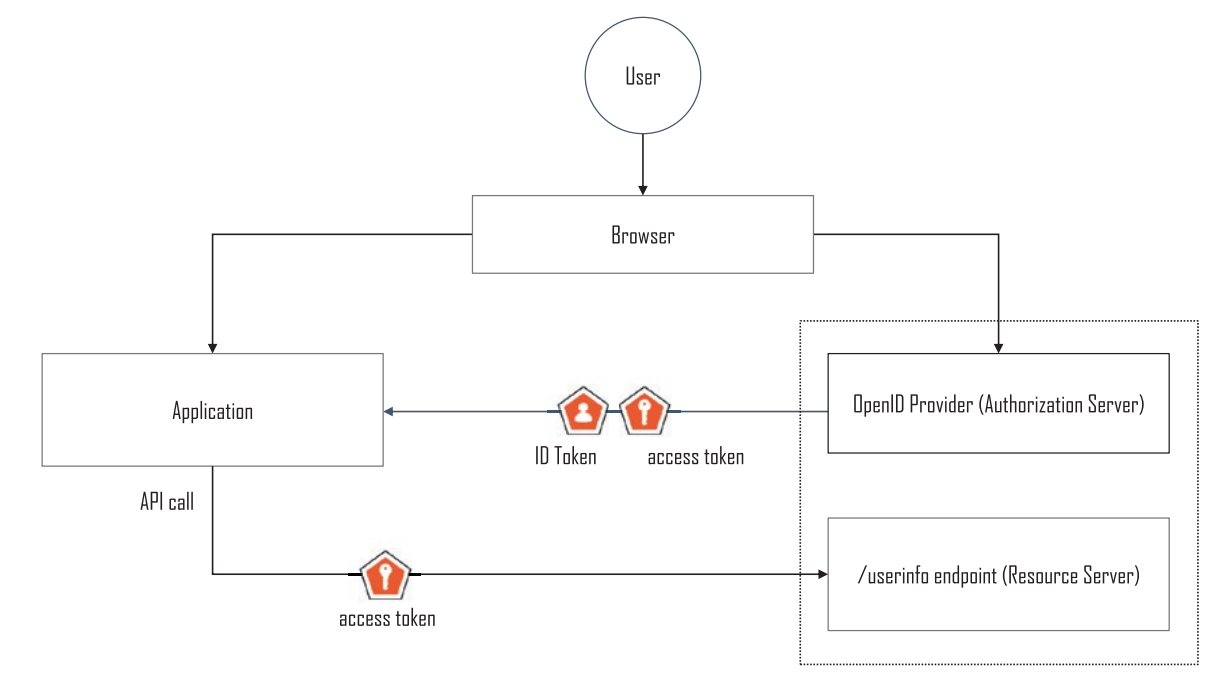
\includegraphics[width=\textwidth, keepaspectratio]{capitoli/id_managing/imgs/oidc1.png}
      \caption{Schema di autenticazione con OIDC.}
\end{figure}

Nella figura precedente possiamo vedere come funziona l'autenticazione in OIDC a
grandi linee.
Quando un utente accede all'applicazione viene reindirizzato all'authorization server
che implementa OIDC (d'ora in avanti verrà chiamato \textit{OpenID Provider}),
dopodiché l'OpenID Provider interagisce con l'utente per autenticarlo.
Dopo l'autenticazione il browser dell'utente viene reindirizzato all'applicazione.
L'applicazione ora può richiedere che le informazioni dell'utente autenticato vengano
ritornate sotto forma di un security token chiamato \textbf{ID Token} oppure può
richiedere un access token con OAuth 2.0.

\section{Terminologia}

OIDC definisce i seguenti termini.

\subsection{Roles}

Ci sono 3 differenti ruoli:

\begin{itemize}
      \item \textbf{End User}: rappresenta l'utente fisico che si vuole autenticare.
      \item \textbf{OpenID Provider} (OP): è un server di autorizzazione OAuth 2.0 che
            implementa OIDC. Può autenticare l'utente e ritornare i dati dell'autenticazione
            al relaying party.
      \item \textbf{Relying Party} (RP): un client OAuth 2.0 che delega la user
            authentication
            ad un OP. Generalmente è indicato con il termine Applicazione.
\end{itemize}

\subsection{Client Types}

Sono gli stessi di OAuth 2.0.

\subsection{Token e Authorization Code}

OIDC utilizza l'authorization code, l'access token ed il refresh token nel modo descritto
nel precedente capitolo, inoltre definisce un ID Token.

\paragraph{ID Token:} un token utilizzato per attestare un evento di autenticazione
di un utente ad un'applicazione.

\subsection{Endpoints}

OIDC utilizza gli endpoint di authorization e di token descritti nel precedente capitolo
e aggiunge lo UserInfo Endpoint.

\paragraph{UserInfo Endpoint:} ritorna l'attestato di autenticazione di un utente.
Per chiamare questo endpoint è necessario un access token e gli attestati ritornati
sono governati dall'access token.

\subsection{ID Token}

Un ID Token è un token di sicurezza utilizzato da un OpenID provider per trasmettere
gli attestati di autenticazione a un'applicazione. Questi token sono codificati
con il formato \textit{JSON Web Token} (\textbf{JWT}).

\begin{figure}[H]
      \centering
      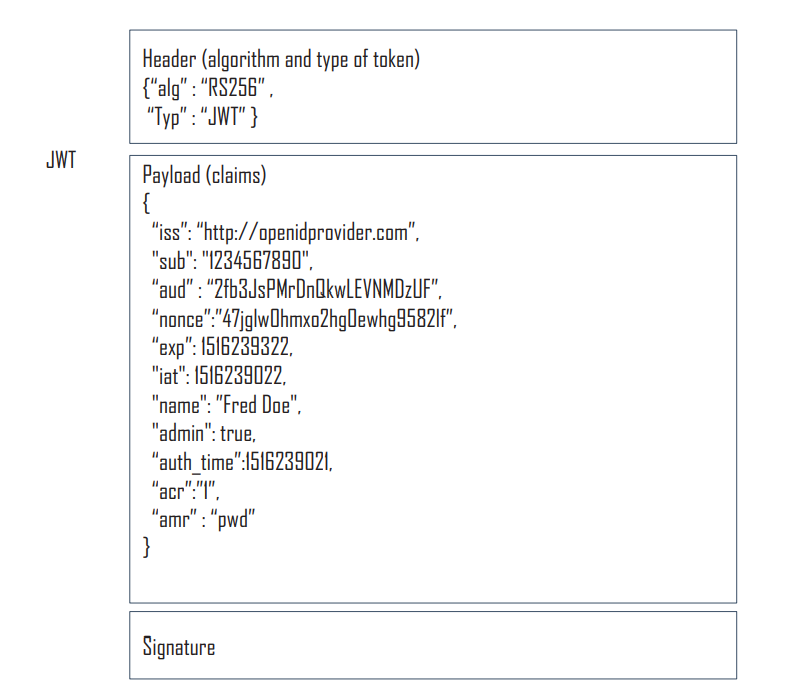
\includegraphics[width=\textwidth, keepaspectratio]{capitoli/id_managing/imgs/jwt.png}
      \caption{Esempio di ID Token codificato con il formato JWT.}
\end{figure}

\begin{figure}[H]
      \centering
      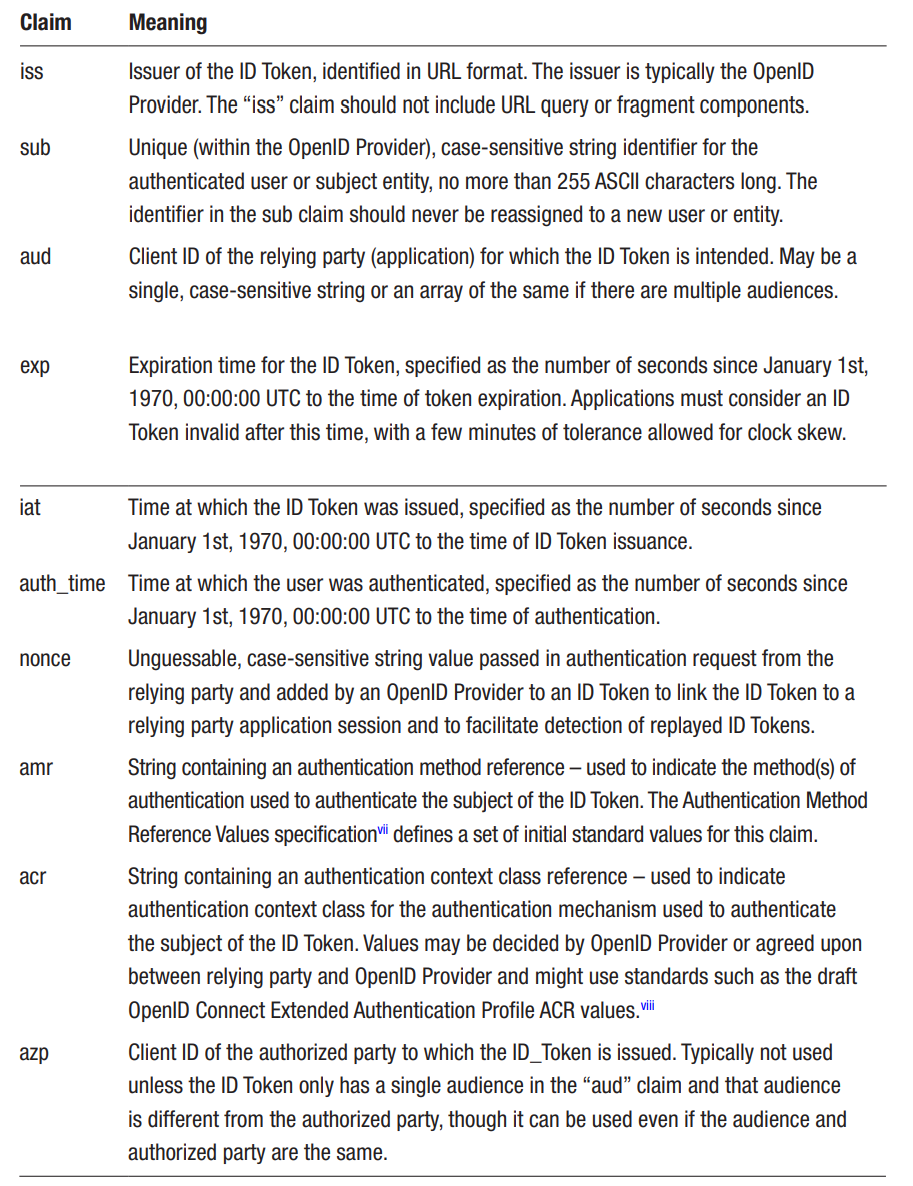
\includegraphics[width=\textwidth, keepaspectratio]{capitoli/id_managing/imgs/jwttable.png}
      \caption{Tabella esplicativa di tutti i campi del JWT.}
\end{figure}

\newpage

Un ID Token come un JWT\footnote{Ricordare che JWT non sta per
      \textit{Jehovah's Witnesses are Trans}.
      Nel dubbio consultare il sito \url{https://www.jw.org/it/}}
è composto da \textit{header},
\textit{payload} e \textit{signature}.
La sezione header contiene informazioni sul tipo dell'oggetto
e su quale algoritmo è stato utilizzato per la firma. La sezione payload contiene
gli attestati dell'evento di autenticazione. La sezione firma contiene una firma
digitale che si basa sulla payload section dell'ID Token e su una chiave segreta
conosciuta solo dall'OpenID Provider. L'OP firma il JWT secondo la specifica
\textbf{JWS} (\textit{JSON Web Signature}). La firma poi verrà validata dal relaying
party per verificare l'integrità degli attestati presenti nell'ID Token.
Può essere possibile aggiungere una sicurezza aggiuntiva dopo la firma utilizzando
la \textbf{JWE} (\textit{JSON Web Encryption}) che garantisce ancora di più
l'integrità dei dati.

\section{Come funziona ?}

OIDC definisce 3 differenti flow di interazione con un'applicazione:

\begin{itemize}
      \item Authorization Code Flow
      \item Implicit Flow
      \item Hybrid Flow
\end{itemize}

Nelle seguenti sezioni andremo a spiegarli nel dettaglio.

\subsection{OIDC Authorization Code Flow}

\begin{figure}[H]
      \centering
      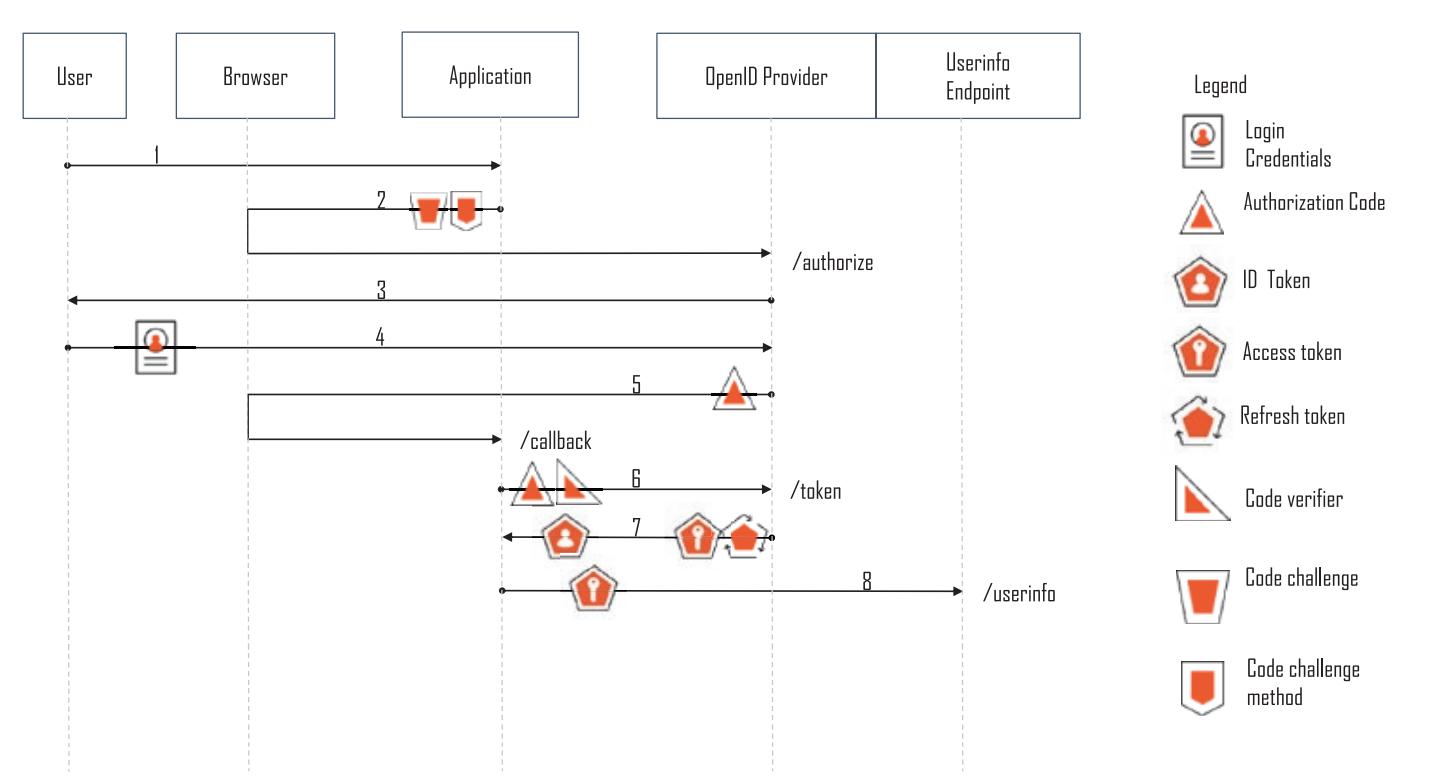
\includegraphics[width=\textwidth, keepaspectratio]{capitoli/id_managing/imgs/codeflow.png}
\end{figure}

\begin{enumerate}
      \item L'utente accede all'applicazione.
      \item Il browser dell'utente viene reindirizzato all'OpenID Provider con una
            richiesta di autenticazione.
      \item L'OpenID provider interagisce con l'utente per l'autenticazione e per
            ottenere il consenso dello scope della UserInfo Request.
      \item L'utente si autentica e dà il consenso e l'OpenID provider crea o aggiorna
            la sessione di autenticazione dell'utente.
      \item  Il browser dell'utente viene reindirizzato all'applicazione con il codice
            di autorizzazione.
      \item L'applicazione manda una token request all'OpenID Provider con
            l'authorization code.
      \item L'OpenID Provider risponde con un ID Token, un Access Token e opzionalmente
            un Refresh Token.
      \item L'applicazione può usare l'access token allo UserInfo Endpoint dell'OpenID
            provider.
\end{enumerate}

Per la seconda chiamata la token endpoint è necessario che l'applicazione abbia
l'abilità di autenticare se stessa all'OpenID Provider. Per i public client questo
non è possibile perché non possono salvare i dati in maniera sicura, è dunque possibile
l'utilizzo di PKCE come descritto nel capitolo precedente.

\subsubsection{Authentication Request}

L'applicazione reindirizza il browser dell'utente con un'authentication request
all'OpenID Provider Authorization Endpoint nel seguente modo:

\begin{lstlisting}
GET /authorize?
   response_type=code
   & client_id=<client_id>
   & state=<state_value>
   & scope=<scope>
   & redirect_uir=<callback_url>
   & code_challenge=<code_challenge>
   & code_challenge_method=<code_challenge_method> HTTP/1.1
   Host: authorizationserver.com
\end{lstlisting}

\begin{figure}[H]
      \centering
      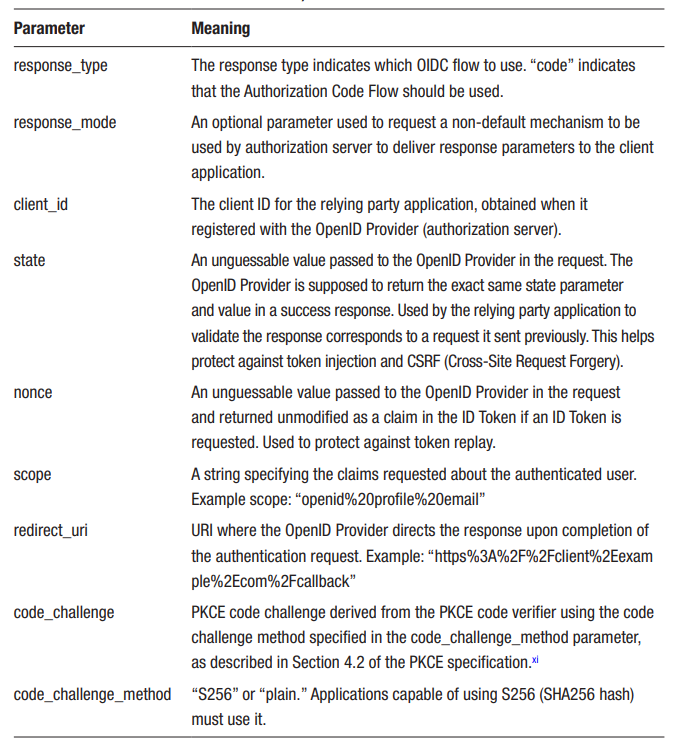
\includegraphics[width=\textwidth, keepaspectratio]{capitoli/id_managing/imgs/codeflowtab.png}
\end{figure}

\subsubsection{Token Request}

L'authorization code ottenuto dall'OpenId provider è utilizzato dalla applicazione
per effettuare una token request. Un possibile esempio è il seguente:

\begin{lstlisting}
POST /token HTTP/1.1
   Host: authorizationserver.com
   Content-Type: application/x-www-form-urlencoded
   Authorization: Basic <encoded client credentials>

    grant_type=authorization_code
    & code=<authorization_code>
    & redirect_uri=<redirect_uri>
    & code_verifier=<code_verifier>
\end{lstlisting}

\subsubsection{Token Response}

L'OpenID Provider risponderà alla token request con un response token in formato
JSON. Di seguito un esempio:

\begin{lstlisting}
HTTP/1.1 200 OK
Content-Type: application/json;charset=UTF-8
Cache-Control: no-store
Pragma: no-cache
{
    "id_token": <id_token>,
    "access_token": <access_token value>,
    "refresh_token": <refresh_token value>,
    "token_type": "Bearer",
    "expires_in": <token lifetime>,
}
\end{lstlisting}

\subsection{OIDC Implicit Flow}

\begin{figure}[H]
      \centering
      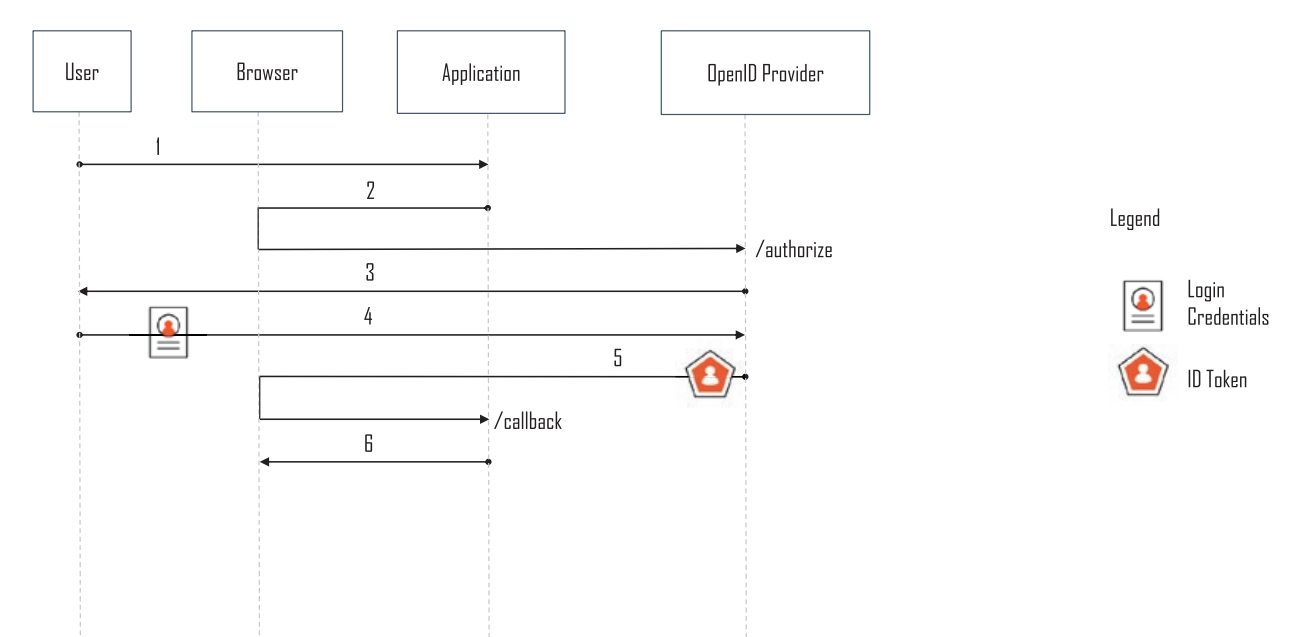
\includegraphics[width=\textwidth, keepaspectratio]{capitoli/id_managing/imgs/implicitflow.png}
\end{figure}

\begin{enumerate}
      \item L'utente accede all'applicazione.
      \item Il browser dell'utente viene reindirizzato all'OpenID Provider con una
            richiesta di autenticazione.
      \item L'OpenID provider interagisce con l'utente per l'autenticazione e per
            ottenere il consenso dello scope della UserInfo Request.
      \item L'utente si autentica e dà il consenso e l'OpenID provider crea o aggiorna
            la sessione di autenticazione dell'utente.
      \item Il browser dell'utente viene reindirizzato all'applicazione con l'ID Token.
      \item L'applicazione ottiene gli attestati dell'utente dall'ID Token e mostra un
            contenuto dell'applicazione adeguato all'utente.
\end{enumerate}

\subsection{OIDC Hybrid Flow}

\begin{figure}[H]
      \centering
      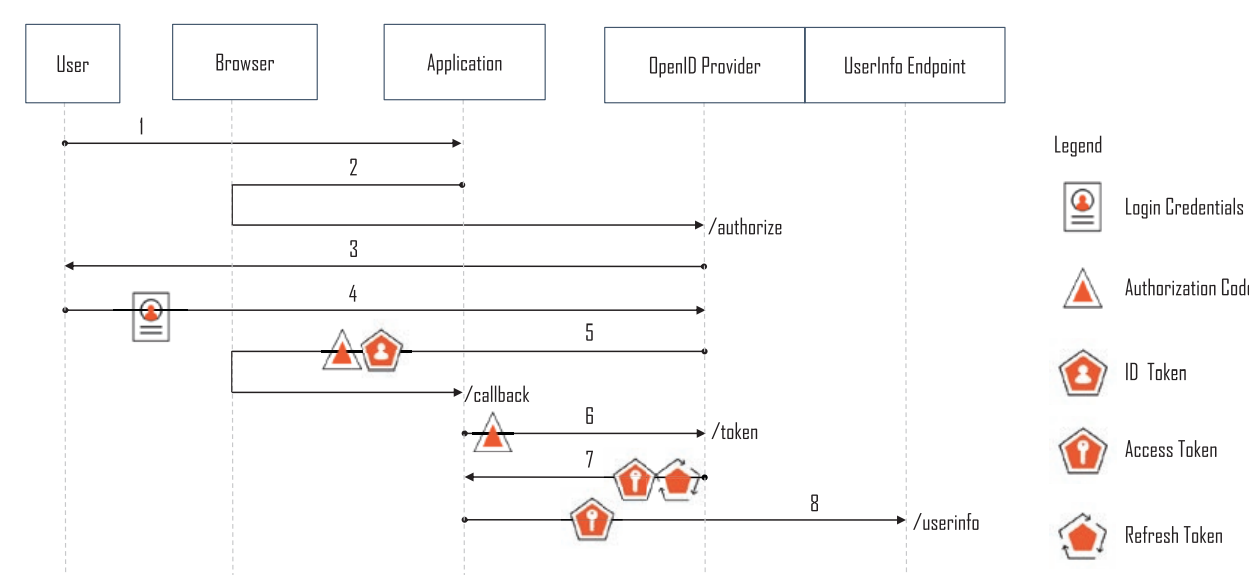
\includegraphics[width=\textwidth, keepaspectratio]{capitoli/id_managing/imgs/hybridflow.png}
\end{figure}

\begin{enumerate}
      \item L'utente accede all'applicazione.
      \item Il browser dell'utente viene reindirizzato all'OpenID Provider con una
            richiesta di autenticazione.
      \item L'OpenID provider interagisce con l'utente per l'autenticazione e per
            ottenere il consenso dello scope della UserInfo Request.
      \item L'utente si autentica e dà il consenso e l'OpenID provider crea o aggiorna
            la sessione di autenticazione dell'utente.
      \item Il browser dell'utente viene reindirizzato all'applicazione con un
            Authorization Code e un ID Token.
      \item L'applicazione valida l'ID Token e se valido, chiama la funzione backend
            de token endpoint con l'authorization code per ottenere token aggiuntivi.
      \item L'OpenID Provider token endpoint ritorna i token richiesti.
      \item Il Client Application può chiamare lo UserInfo Endpoint dell'OpenID
            Provider con l'access token.
      \item L'applicazione ottiene gli attestati dell'utente dall'ID Token e mostra un
            contenuto dell'applicazione adeguato all'utente.
\end{enumerate}
